\documentclass[letterpaper,12pt]{article}
\usepackage[utf8]{inputenc}
\usepackage[german]{babel}
\usepackage{amsmath}
\usepackage{amssymb}
\usepackage{latexsym}
\usepackage{xcolor}
\usepackage{dsfont}
\usepackage{amsfonts}
\usepackage{array} 
\usepackage{multirow}
\usepackage{vmargin}
\usepackage{fancyhdr}
\usepackage{graphicx}
\pagestyle{fancy}

\setmargins{2.5cm}{1.5cm}{16.5cm}{23.42cm}{10pt}{1cm}{0pt}{2cm}

\title{Problemas físicos}
\author{César Eduardo Rosete}
\date{Noviembre 2022}

\begin{document}

\maketitle
\lhead{\leftmark}
\chead{César Eduardo Rosete Gómez}
\rhead{\thepage}
\lfoot{\leftmark}
\rfoot{\thepage}
\section*{Problema 1}
Sabiendo que las definiciones de velocidad y aceleración son:
\begin{align}
    \Vec{v}&=\frac{dx}{dt}\\
    \Vec{a}&=\frac{d\Vec{v}}{dt}
\end{align}
Dadas las definiciones de derivadas, i.e. un cambio sumamente pequeño; de (2) podemos decir:
\begin{align*}
    \Vec{a}*t&=d\Vec{v}\\
    \Vec{a}*t&=\Vec{v_f}-\Vec{v_0}\\
    \Vec{a}*t+\Vec{v_0}&=\Vec{v_f}
\end{align*}
Ahora si integramos ambos lados:
\begin{align*}
    \int \Vec{a}*t+\Vec{v_0} dt&=\int \Vec{v_f}dt\\
    \frac{1}{2}*\Vec{a}*t^2+\Vec{v_0}t &=\Vec{v_f}*t\\
\end{align*}
Pero por (1) sabemos que $\Vec{v}=\frac{dx}{dt}$ entonces se sigue:
\begin{align*}
    \Delta x&=\frac{1}{2}*\Vec{a}*t^2+\Vec{v_0}*t 
    x-x_0=\frac{1}{2}*\Vec{a}*t^2+\Vec{v_0}*t 
    x=\frac{1}{2}*\Vec{a}*t^2+\Vec{v_0}*t+x_0
\end{align*}
Reorganizando los términos tenemos:
\begin{equation}
    x=x_0+\Vec{v_0}*t+\frac{1}{2}*\Vec{a}*t^2
\end{equation}
\section*{Promblema 2}
\subsection*{a)}
Del problema 1 retomamos (3). De tal manera que:
\begin{align}
    x_{C_1}&=x_{C_1}_0+\Vec{v_{C_1}_0}*t+\frac{1}{2}*\Vec{a_{C_1}}*t^2\\
    x_{C_2}&=x_{C_2}_0+\Vec{v_{C_2}_0}*t+\frac{1}{2}*\Vec{a_{C_2}}*t^2
\end{align}
Sustituyendo los valores dados en (4) y (5) en $t=t_0$ considerando $t_0$ el momento en el que parte el segundo carro:
\begin{align}
    x_{C_1}&=1.75+3.5*t+\frac{1}{2}*3.5*t^2\\
    x_{C_2}&=0+0*t+\frac{1}{2}*4.9*t^2
\end{align}
Igualando las posiciones $x_{C_1}$ y $x_{C_2}$ se obtiene:
\begin{align}
    1.75+3.5*t+\frac{1}{2}*3.5*t^2&=0+0*t+\frac{1}{2}*4.9*t^2\\
    1.75+3.5*t+\frac{1}{2}*3.5*t^2&=\frac{1}{2}*4.9*t^2\\
    1.75+3.5*t+&=\frac{1}{2}*1.4*t^2\\
    \frac{1}{2}*1.4*t^2-3.5*t-1.75&=0\\
\end{align}
Por la fórmula del chicharonero se obtiene:
 \begin{align*}
      x&=\frac{-b\pm\sqrt{b^2-4ac}}{2a}\\
      x&=\frac{3.5\pm\sqrt{(-3.5)^2-4(\frac{1.4}{2})(-1.75)}}{2(\frac{1.4}{2})}\\
      x&=\frac{3.5\pm\sqrt{(3.5)^2+4(\frac{1.4}{2})(1.75)}}{2(\frac{1.4}{2})}
 \end{align*}
 De donde se obtiene
 \begin{align*}
     x_1=\frac{5+\sqrt{35}}{2}\\
     x_2=\frac{5-\sqrt{35}}{2}\\
 \end{align*}
 El valor que nos interesa en este caso es $x_1$\\
 :. El carro 2 alcanza al carro 1 a los 5.46 s
 \subsection*{b)}
 De evaluar en  a),(6) se obtiene que x=73 m
 \subsection*{c)}
 Retomando del problema 1, del desarrollo de (2) sabemos que:
 \begin{equation}
      \Vec{a}*t+\Vec{v_0}&=\Vec{v_f}
 \end{equation}
 Sustituyendo para $ C_1$ obtenemos que $\Vec{v_{C_1}_f}=22.61\frac{m}{s}$.\\
 Por otro lado, para $C_2$ obtenemos que $\Vec{v_{C_2}_f}=26.75\frac{m}{s}$.
 \subsection*{d)}
 \begin{table}[h]
    \centering
    \begin{tabular}{c|c|c|c}\hline\hline
    \multicolumn{4}{c}{Carro 1} \\\hline
    No dependientes del tiempo & \multicolumn{3}{c}{Dependientes del tiempo} \\\hline
    a[m/s^2]&t[s]&x[m]&v[m/s]\\\hline
    3.5&2&15.75&10.5\\\hline
    3.5&3&28&14\\\hline
    3.5&4&43.75&17.5\\\hline
    3.5&6&85.75&24.5\\\hline
    3.5&7&112&28\\\hline
    \end{tabular}
    \caption{Cinética carro 1}
    \label{tab: Cuadro1}
\end{table}
\begin{table}[h]
    \centering
    \begin{tabular}{c|c|c|c}\hline\hline
    \multicolumn{4}{c}{Carro 2} \\\hline
    No dependientes del tiempo & \multicolumn{3}{c}{Dependientes del tiempo} \\\hline
    a[m/s^2]&t[s]&x[m]&v[m/s]\\\hline
    4.9&2&9.8&9.8\\\hline
    4.9&3&22.05&14.7\\\hline
    4.9&4&39.2&19.6\\\hline
    4.9&6&88.2&29.4\\\hline
    4.9&7&120.05&34.3\\\hline\hline
    \end{tabular}
    \caption{Cinética carro 2}
    \label{tabla: Cuadro1}
\end{table}
\section*{Problema 3}
\begin{figure}[htb]
    \centering
    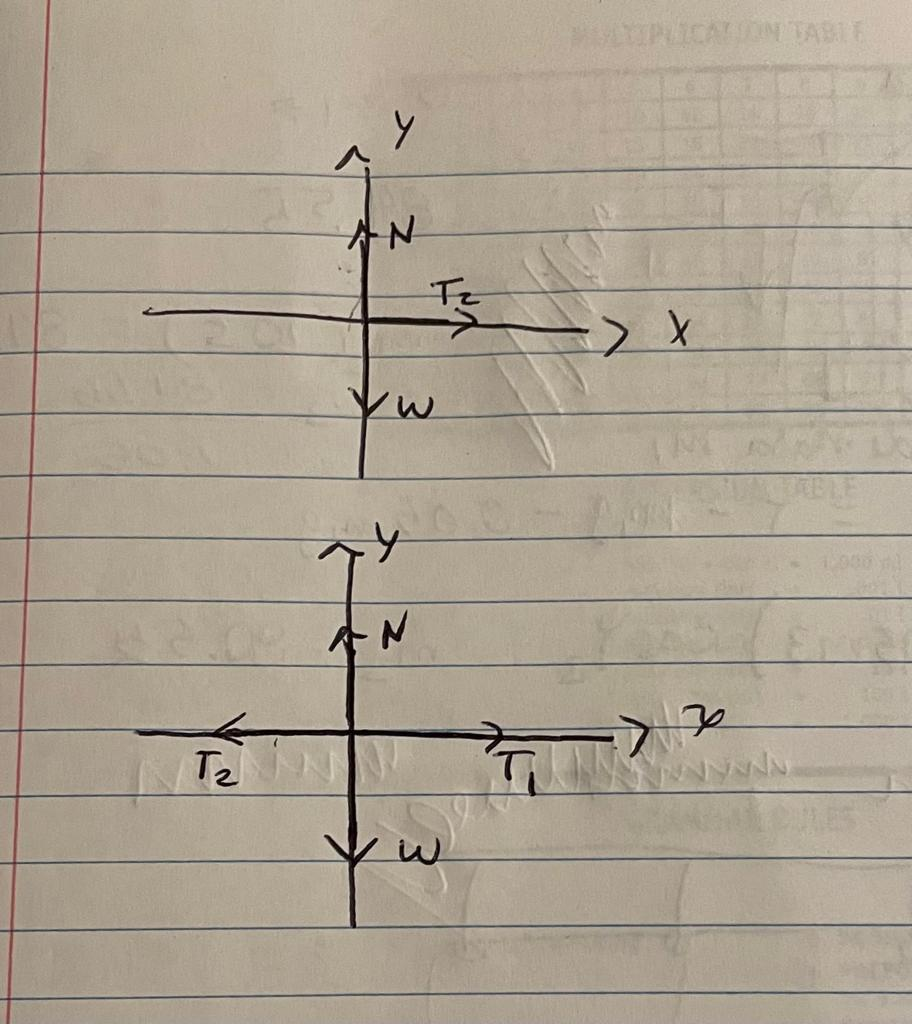
\includegraphics[width=6cm,height=6cm]{Imagenes/Diagramas_cl.jpeg}
    \caption{La imagen son los diagramas de flujo del cuerpo de masa $m_1$ y $m_2$ de forma decendente respectivamente}
    \label{Imagen:Diagramas de flujo }
\end{figure}
Por la fórmula $\Vec{F}=m\Vec{a}$ podemos decir que el problema consiste de dos componentes, pues hay una serie de fuerzas que afectan a los cuerpos sobre el eje vertical y otra que afecta a los cuerpos de manera horizontal.\\
Debido a que en el sistema no hay friccíon, sabemos que $\sum \Vec{F_y}=0$.\\
Por otro lado, podemos observar que en el eje X la suma no es necesariamente igual a cero, por lo que tenemos:
\begin{equation*}
    \sum \Vec{F_x}=A-T_1-T_2
\end{equation*}
Por esta ecuación y la tercera ley de Newton podemos decir que:
\begin{align*}
    \sum \Vec{F_x}=(m_1+m_2)*\Vec{a}\\
    \Vec{a}=\frac{\sum \Vec{F_x}}{(m_1+m_2)}
\end{align*}

\end{document}
